\newpage
\section{Testowanie programu}
Poszczególne funkcjonalności programu zostały przetestowane za pomocą testów jednostkowych (ang. \emph{unit test}). Testy dotyczące danych funkcji są zawarte w module \emph{mod test}, w tym samym pliku źródłowym oraz bazują na wbudowanej infrastrukturze testowej ekosystemu języka \emph{Rust}. Aby uruchomić wszystkie testy wystarczy użyć komendy \emph{cargo test} w głównym folderze projektu. Zrzut ekranu, przedstawiający pozytywny wynik wszystkich testów, zawarto na rysunku \ref{regression}.

\begin{figure}[h]
\center
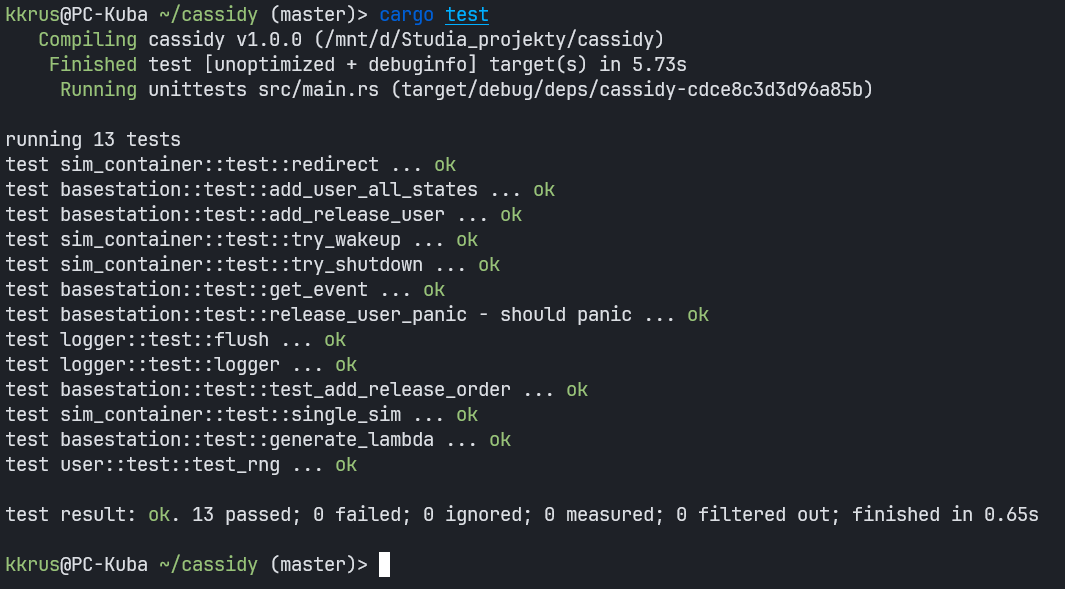
\includegraphics[scale=0.55]{img/tests.png} 
\caption{Przykładowy wynik komendy \emph{cargo test}}
\label{regression}
\end{figure}

\noindent W procesie testowania aplikacji wykorzystywano także generowane pliki \emph{log} oraz wymienione w sekcji \ref{python_scripts} skrypty napisane w języku \emph{Python}. Umożliwiają one ręczne oraz automatyczne sprawdzanie poprawności działania pętli głównej programu. Fragment przykładowego pliku \emph{event log} przedstawiono poniżej. Pierwsza kolumna zawiera znacznik czasu wyrażony w mikrosekundach. Następnie podany jest rodzaj zdarzenia oraz dotyczące go informacje.

\begin{verbatim}
10009189   UserAdd       Station id: 2   User id: 14, end time: 12492641 next user: 11003934
10941299   UserRelease   Station id: 0   User id: 3, end time: 10941299
11003934   UserAdd       Station id: 2   User id: 15, end time: 17544415 next user: 17034435
11161844   UserRelease   Station id: 0   User id: 5, end time: 11161844
12097745   UserAdd       Station id: 0   User id: 16, end time: 36047089 next user: 13170839
12492641   UserRelease   Station id: 2   User id: 14, end time: 12492641
13100375   UserRelease   Station id: 2   User id: 1, end time: 13100375
13170839   UserAdd       Station id: 0   User id: 17, end time: 34192635 next user: 14459706
14299594   UserRelease   Station id: 0   User id: 8, end time: 14299594
\end{verbatim}

